\documentclass[aspectratio=169]{beamer}
\usetheme{Madrid}
\usecolortheme{default}

% Packages
\usepackage{graphicx}
\usepackage{amsmath}
\usepackage{amssymb}
\usepackage{algorithm}
\usepackage{algorithmic}
\usepackage{tikz}
\usepackage{booktabs}
\usepackage{multirow}
\usepackage{xcolor}

% Custom colors
\definecolor{darkblue}{RGB}{0,51,102}
\definecolor{lightblue}{RGB}{51,153,255}
\definecolor{darkgreen}{RGB}{0,102,51}

\setbeamercolor{structure}{fg=darkblue}
\setbeamercolor{frametitle}{bg=darkblue,fg=white}
\setbeamercolor{title}{bg=darkblue,fg=white}

% Remove navigation symbols
\setbeamertemplate{navigation symbols}{}

% Footer
\setbeamertemplate{footline}{
  \leavevmode%
  \hbox{%
  \begin{beamercolorbox}[wd=.333333\paperwidth,ht=2.25ex,dp=1ex,center]{author in head/foot}%
    \usebeamerfont{author in head/foot}\insertshortauthor
  \end{beamercolorbox}%
  \begin{beamercolorbox}[wd=.333333\paperwidth,ht=2.25ex,dp=1ex,center]{title in head/foot}%
    \usebeamerfont{title in head/foot}\insertshorttitle
  \end{beamercolorbox}%
  \begin{beamercolorbox}[wd=.333333\paperwidth,ht=2.25ex,dp=1ex,right]{date in head/foot}%
    \usebeamerfont{date in head/foot}\insertshortdate{}\hspace*{2em}
    \insertframenumber{} / \inserttotalframenumber\hspace*{2ex} 
  \end{beamercolorbox}}%
  \vskip0pt%
}

% Title information
\title[Verifiable Byzantine Robust GNNs in FL]{Verifiable Byzantine Robust Graph Neural Networks using Federated Learning}
\author[Tawkir, Nobo]{2005090 - Tawkir Aziz Rahman \\ 2005074 - Dipanto Kumar Roy Nobo}
\institute[BUET]{CSE472: Machine Learning Sessional \\ Department of Computer Science and Engineering \\ Bangladesh University of Engineering and Technology (BUET)}
\date[December 2025]{December 2025}

\begin{document}

%%%%%%%%%%%%%%%%%%%%%%%%%%%%%%%%%%%%%%%%%%%%%%%%%
% Slide 1: Title Slide
%%%%%%%%%%%%%%%%%%%%%%%%%%%%%%%%%%%%%%%%%%%%%%%%%
\begin{frame}
	\titlepage
\end{frame}

%%%%%%%%%%%%%%%%%%%%%%%%%%%%%%%%%%%%%%%%%%%%%%%%%
% Slide 2: Problem & Motivation
%%%%%%%%%%%%%%%%%%%%%%%%%%%%%%%%%%%%%%%%%%%%%%%%%
\begin{frame}{Problem \& Motivation}

	\begin{block}{Problem Statement}
		Training AI models on graph data across multiple organizations is challenging due to security threats and privacy concerns.
	\end{block}


	\begin{columns}[T]
		\begin{column}{0.48\textwidth}
			\textbf{Key Challenges:}
			\begin{itemize}
				\item \textbf{Privacy}: Organizations can't share sensitive data
				\item \textbf{Security}: Malicious participants can corrupt the model
				\item \textbf{Trust}: Hard to verify if participants are honest
			\end{itemize}
		\end{column}

		\begin{column}{0.48\textwidth}
			\textbf{Real-World Applications:}
			\begin{itemize}
				\item \textcolor{darkgreen}{Healthcare}: Disease networks across hospitals
				\item \textcolor{darkgreen}{Finance}: Fraud detection across banks
				\item \textcolor{darkgreen}{Social Networks}: Privacy-preserving analysis
				\item \textcolor{darkgreen}{Cybersecurity}: Distributed threat detection
			\end{itemize}
		\end{column}
	\end{columns}

	\begin{alertblock}{Our Goal}
		Develop a secure and verifiable system for collaborative graph-based machine learning.
	\end{alertblock}

\end{frame}

%%%%%%%%%%%%%%%%%%%%%%%%%%%%%%%%%%%%%%%%%%%%%%%%%
% Slide 3: Background & Related Work
%%%%%%%%%%%%%%%%%%%%%%%%%%%%%%%%%%%%%%%%%%%%%%%%%
\begin{frame}{Background \& Related Work}
	\small
	\begin{columns}[T]
		\begin{column}{0.48\textwidth}
			\textbf{Foundation: RUNG (NeurIPS 2024)}
			\begin{itemize}
				\item Robust method for handling graph data
				\item Reduces bias in predictions
				\item Strong performance guarantees
			\end{itemize}


			\textbf{Why RUNG?}
			\begin{itemize}
				\item State-of-the-art robustness
				\item Handles noisy connections effectively
				\item Proven theoretical guarantees
			\end{itemize}

		\end{column}

		\begin{column}{0.48\textwidth}
			\textbf{Collaborative Learning Challenges}
			\begin{itemize}
				\item \textbf{Malicious Participants}: Some clients may be dishonest
				\item \textbf{Data Diversity}: Different data distributions across clients
				\item \textbf{Efficiency}: Need to minimize communication overhead
			\end{itemize}

			\textbf{Existing Defense Methods}
			\begin{itemize}
				\item Distance-based filtering
				\item Statistical aggregation
				\item Averaging techniques
			\end{itemize}



		\end{column}
	\end{columns}
	\begin{alertblock}{Limitation}
		Current methods don't work well with graph data and lack verification.
	\end{alertblock}
\end{frame}

%%%%%%%%%%%%%%%%%%%%%%%%%%%%%%%%%%%%%%%%%%%%%%%%%
% Slide 4: Proposed Approach (Part 1)
%%%%%%%%%%%%%%%%%%%%%%%%%%%%%%%%%%%%%%%%%%%%%%%%%
\begin{frame}{Proposed Approach: System Architecture}
	\small
	\begin{center}
		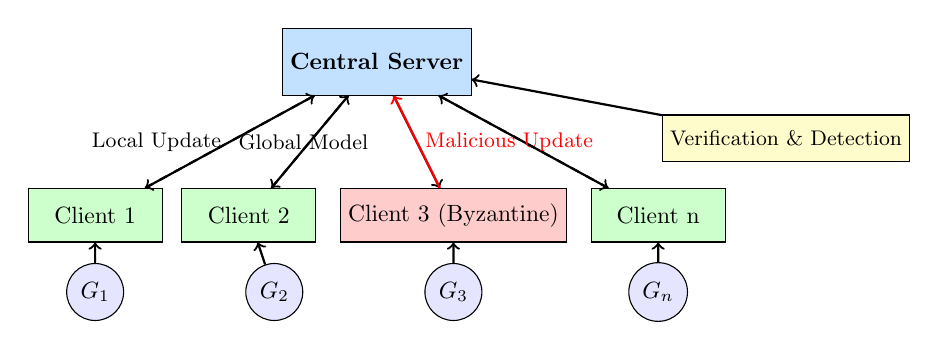
\begin{tikzpicture}[scale=0.65, every node/.style={scale=0.85}]
			% Server
			\node[draw, rectangle, fill=lightblue!30, minimum width=2.5cm, minimum height=1cm] (server) at (0,4) {\textbf{Central Server}};

			% Clients
			\node[draw, rectangle, fill=green!20, minimum width=2cm, minimum height=0.8cm] (client1) at (-5.5,1) {Client 1};
			\node[draw, rectangle, fill=green!20, minimum width=2cm, minimum height=0.8cm] (client2) at (-2.5,1) {Client 2};
			\node[draw, rectangle, fill=red!20, minimum width=2cm, minimum height=0.8cm] (client3) at (1.5,1) {Client 3 (Byzantine)};
			\node[draw, rectangle, fill=green!20, minimum width=2cm, minimum height=0.8cm] (client4) at (5.5,1) {Client n};

			% Local graphs
			\node[draw, circle, fill=blue!10, minimum size=0.6cm] (g1) at (-5.5,-0.5) {$G_1$};
			\node[draw, circle, fill=blue!10, minimum size=0.6cm] (g2) at (-2,-0.5) {$G_2$};
			\node[draw, circle, fill=blue!10, minimum size=0.6cm] (g3) at (1.5,-0.5) {$G_3$};
			\node[draw, circle, fill=blue!10, minimum size=0.6cm] (g4) at (5.5,-0.5) {$G_n$};

			% Arrows
			\draw[->, thick] (server) -- node[right] {\small Global Model} (client1);
			\draw[->, thick] (server) -- (client2);
			\draw[->, thick] (server) -- (client3);
			\draw[->, thick] (server) -- (client4);

			\draw[->, thick, dashed] (client1) -- node[left] {\small Local Update} (server);
			\draw[->, thick, dashed] (client2) -- (server);
			\draw[->, thick, red] (client3) -- node[right] {\small Malicious Update} (server);
			\draw[->, thick, dashed] (client4) -- (server);

			\draw[->, thick] (g1) -- (client1);
			\draw[->, thick] (g2) -- (client2);
			\draw[->, thick] (g3) -- (client3);
			\draw[->, thick] (g4) -- (client4);

			% Verification box
			\node[draw, rectangle, fill=yellow!20, minimum width=2.5cm, minimum height=0.7cm] (verify) at (8,2.5) {\small Verification \& Detection};
			\draw[->, thick] (verify) -- (server);
		\end{tikzpicture}
	\end{center}


	\begin{block}{Key Components}
		\begin{enumerate}
			\item \textbf{Local Training}: Each client trains RUNG on local graph $G_i$
			\item \textbf{Verifiable Aggregation}: Cryptographic proofs ensure correct local computation
			\item \textbf{Byzantine Detection}: Statistical tests identify malicious clients
			\item \textbf{Robust Update}: Weighted aggregation down-weights suspicious updates
		\end{enumerate}
	\end{block}

\end{frame}

%%%%%%%%%%%%%%%%%%%%%%%%%%%%%%%%%%%%%%%%%%%%%%%%%
% Slide 5: Proposed Approach (Part 2)
%%%%%%%%%%%%%%%%%%%%%%%%%%%%%%%%%%%%%%%%%%%%%%%%%
\begin{frame}{Proposed Approach: Key Innovations}

	\begin{columns}[T]
		\begin{column}{0.48\textwidth}

			\textbf{1. Verifiable Training}
			\begin{itemize}
				\item Each client provides cryptographic proof of honest computation
				\item Server can verify correctness without accessing private data
				\item Fast and efficient verification process
			\end{itemize}


			\begin{block}{Benefits}
				\begin{itemize}
					\item Ensures data privacy
					\item Detects dishonest behavior
					\item Low computational overhead
				\end{itemize}
			\end{block}

		\end{column}

		\begin{column}{0.48\textwidth}

			\textbf{2. Malicious Client Detection}
			\begin{itemize}
				\item Compare updates from different clients
				\item Identify suspicious or outlier behavior
				\item Automatically down-weight malicious contributions
			\end{itemize}


			\begin{block}{Aggregation Strategy}
				\begin{itemize}
					\item Trusted clients get higher weight
					\item Suspicious clients are excluded
					\item Adaptive to attack patterns
				\end{itemize}
			\end{block}

		\end{column}
	\end{columns}


	\begin{alertblock}{Guarantee}
		Our system remains accurate even when up to 30\% of participants are malicious.
	\end{alertblock}

\end{frame}

%%%%%%%%%%%%%%%%%%%%%%%%%%%%%%%%%%%%%%%%%%%%%%%%%
% Slide 6: Experimental Plan
%%%%%%%%%%%%%%%%%%%%%%%%%%%%%%%%%%%%%%%%%%%%%%%%%
\begin{frame}{Experimental Plan}

	\begin{columns}[T]
		\begin{column}{0.48\textwidth}

			\textbf{Benchmark Datasets}
			\begin{itemize}
				\item Cora - Small academic citation network
				\item CiteSeer - Medium citation network
				\item PubMed - Large biomedical network
				\item ogbn-arxiv - Very large academic network
			\end{itemize}


			\textbf{Testing Scenarios}
			\begin{itemize}
				\item Vary number of clients (10 to 50)
				\item Test with different malicious ratios (0\% to 40\%)
				\item Simulate realistic data distributions
			\end{itemize}

		\end{column}

		\begin{column}{0.48\textwidth}

			\textbf{Comparison Methods}
			\begin{itemize}
				\item Standard federated learning
				\item Existing robust methods
				\item Centralized training (ideal case)
			\end{itemize}

			\textbf{What We'll Measure}
			\begin{itemize}
				\item Prediction accuracy under attacks
				\item Ability to detect malicious clients
				\item Communication efficiency
				\item Training speed and convergence
			\end{itemize}

		\end{column}
	\end{columns}

	\begin{block}{Additional Analysis}
		We will study the impact of verification overhead and detection sensitivity.
	\end{block}

\end{frame}

%%%%%%%%%%%%%%%%%%%%%%%%%%%%%%%%%%%%%%%%%%%%%%%%%
% Slide 7: Timeline & Expected Contributions
%%%%%%%%%%%%%%%%%%%%%%%%%%%%%%%%%%%%%%%%%%%%%%%%%
\begin{frame}{Expected Contributions}




	\textbf{Expected Outcomes}

	\vspace{0.3cm}

	\begin{enumerate}
		\item A novel secure training system
		\item Strong performance guarantees
		\item Comprehensive experimental validation
		\item Open-source code release
	\end{enumerate}

	\vspace{0.5cm}

	\begin{block}{Publication Target}
		NeurIPS 2026
	\end{block}

	\vspace{0.3cm}

	\begin{alertblock}{Impact}
		Enables secure collaboration for sensitive graph data across organizations.
	\end{alertblock}


\end{frame}

%%%%%%%%%%%%%%%%%%%%%%%%%%%%%%%%%%%%%%%%%%%%%%%%%
% Backup slide - References (Optional)
%%%%%%%%%%%%%%%%%%%%%%%%%%%%%%%%%%%%%%%%%%%%%%%%%
% \begin{frame}[noframenumbering]{References}

% \footnotesize

% \begin{thebibliography}{99}

% \bibitem{rung2024}
% Hou, Z., Feng, R., Derr, T., \& Liu, X. (2024).
% \newblock Robust Graph Neural Networks via Unbiased Aggregation.
% \newblock \textit{Advances in Neural Information Processing Systems (NeurIPS)}, 37.

% \bibitem{fedavg}
% McMahan, B., et al. (2017).
% \newblock Communication-Efficient Learning of Deep Networks from Decentralized Data.
% \newblock \textit{AISTATS}.

% \bibitem{byzantine}
% Blanchard, P., et al. (2017).
% \newblock Machine Learning with Adversaries: Byzantine Tolerant Gradient Descent.
% \newblock \textit{NeurIPS}.

% \bibitem{krum}
% Blanchard, P., et al. (2017).
% \newblock Byzantine-Tolerant Machine Learning.
% \newblock \textit{arXiv preprint}.

% \bibitem{gnn_attack}
% Zügner, D., et al. (2018).
% \newblock Adversarial Attacks on Neural Networks for Graph Data.
% \newblock \textit{KDD}.

% \end{thebibliography}

% \end{frame}

\end{document}